\documentclass[a4paper,12pt]{article}
\usepackage[utf8]{inputenc}
\usepackage[T2A]{fontenc}
\usepackage[russian]{babel}
\usepackage{geometry}
\usepackage{graphicx}
\usepackage{amsmath}
\usepackage{amsfonts}
\usepackage{hyperref}
\usepackage{array}
\usepackage{longtable}
\usepackage{booktabs}
\usepackage{caption}

\geometry{top=2cm, bottom=2cm, left=2.5cm, right=1.5cm}

\title{Практическая работа 1 по курсу\\"Базы данных"\\Вариант 7\\Модель "Заказ билетов"}
\author{Мурадян Артём Андреевич\\БПМ232}
\date{\today}

\begin{document}

\maketitle
\newpage

\tableofcontents
\newpage

\section{Описание таблиц}

\subsection{Концептуальная описание}
Наша БД состоит из следующих сущностей:
\begin{itemize}
    \item \textbf{Пассажир (Passenger)} — информация о людях, которые летят.
    \item \textbf{Рейс (Flight)} — информация о конкретном рейсе (номер, маршрут, время, самолет).
    \item \textbf{Тип самолета (AircraftType)} — справочник моделей самолетов.
    \item \textbf{Тип рейса (FlightType)} — справочник (регулярный, чартер, специальный).
    \item \textbf{Билет (Ticket)} — связь между пассажиром и рейсом, содержит место и статус.
\end{itemize}

\subsection{Описание таблиц}

\begin{longtable}{|p{3cm}|p{3cm}|p{2.5cm}|p{6cm}|}
\caption{Описание таблиц базы данных} \label{tab:tables} \\
\hline
\textbf{Имя атрибута} & \textbf{Тип атрибута} & \textbf{Ограничение} & \textbf{Описание атрибута} \\
\hline
\endfirsthead

\hline
\textbf{Имя атрибута} & \textbf{Тип атрибута} & \textbf{Ограничение} & \textbf{Описание атрибута} \\
\hline
\endhead

\multicolumn{4}{|c|}{\textbf{Таблица Passenger (Пассажиры)}} \\
\hline
passenger\_id & INTEGER & SERIAL PRIMARY KEY & Уникальный идентификатор пассажира \\
last\_name & VARCHAR(100) & NOT NULL & Фамилия \\
first\_name & VARCHAR(100) & NOT NULL & Имя \\
patronymic & VARCHAR(100) &  & Отчество \\
passport\_number & VARCHAR(20) & UNIQUE NOT NULL & Номер паспорта \\
birth\_date & DATE & NOT NULL & Дата рождения \\
\hline

\multicolumn{4}{|c|}{\textbf{Таблица AircraftType (Типы самолетов)}} \\
\hline
aircraft\_type\_id & INTEGER & SERIAL PRIMARY KEY & Идентификатор типа \\
model & VARCHAR(50) & UNIQUE NOT NULL & Модель самолета \\
manufacturer & VARCHAR(50) & NOT NULL & Производитель \\
capacity & INTEGER & NOT NULL CHECK (capacity > 0) & Количество мест \\
\hline

\multicolumn{4}{|c|}{\textbf{Таблица FlightType (Типы рейсов)}} \\
\hline
flight\_type\_id & INTEGER & SERIAL PRIMARY KEY & Идентификатор типа \\
type\_name & VARCHAR(50) & UNIQUE NOT NULL & Название типа \\
\hline

\multicolumn{4}{|c|}{\textbf{Таблица Flight (Рейсы)}} \\
\hline
flight\_id & INTEGER & SERIAL PRIMARY KEY & Уникальный идентификатор рейса \\
flight\_number & VARCHAR(10) & NOT NULL & Номер рейса \\
departure\_city & VARCHAR(100) & NOT NULL & Город отправления \\
arrival\_city & VARCHAR(100) & NOT NULL & Город прибытия \\
departure\_time & TIMESTAMP & NOT NULL & Дата и время вылета \\
arrival\_time & TIMESTAMP & NOT NULL & Дата и время прилета \\
aircraft\_type\_id & INTEGER & REFERENCES AircraftType(aircraft\_type\_id) & Тип самолета \\
flight\_type\_id & INTEGER & REFERENCES FlightType(flight\_type\_id) & Тип рейса \\
\hline

\multicolumn{4}{|c|}{\textbf{Таблица Ticket (Билеты)}} \\
\hline
ticket\_id & INTEGER & SERIAL PRIMARY KEY & Уникальный номер билета \\
passenger\_id & INTEGER & REFERENCES Passenger(passenger\_id) ON DELETE CASCADE & Пассажир \\
flight\_id & INTEGER & REFERENCES Flight(flight\_id) ON DELETE CASCADE & Рейс \\
seat\_number & VARCHAR(5) &  & Номер места \\
is\_return\_ticket & BOOLEAN & DEFAULT FALSE & Признак обратного билета \\
purchase\_date & TIMESTAMP & DEFAULT CURRENT\_TIMESTAMP & Дата покупки \\
ticket\_status & VARCHAR(20) & DEFAULT 'Куплен' & Статус \\
\hline
\end{longtable}

\begin{figure}[p]
    \centering
    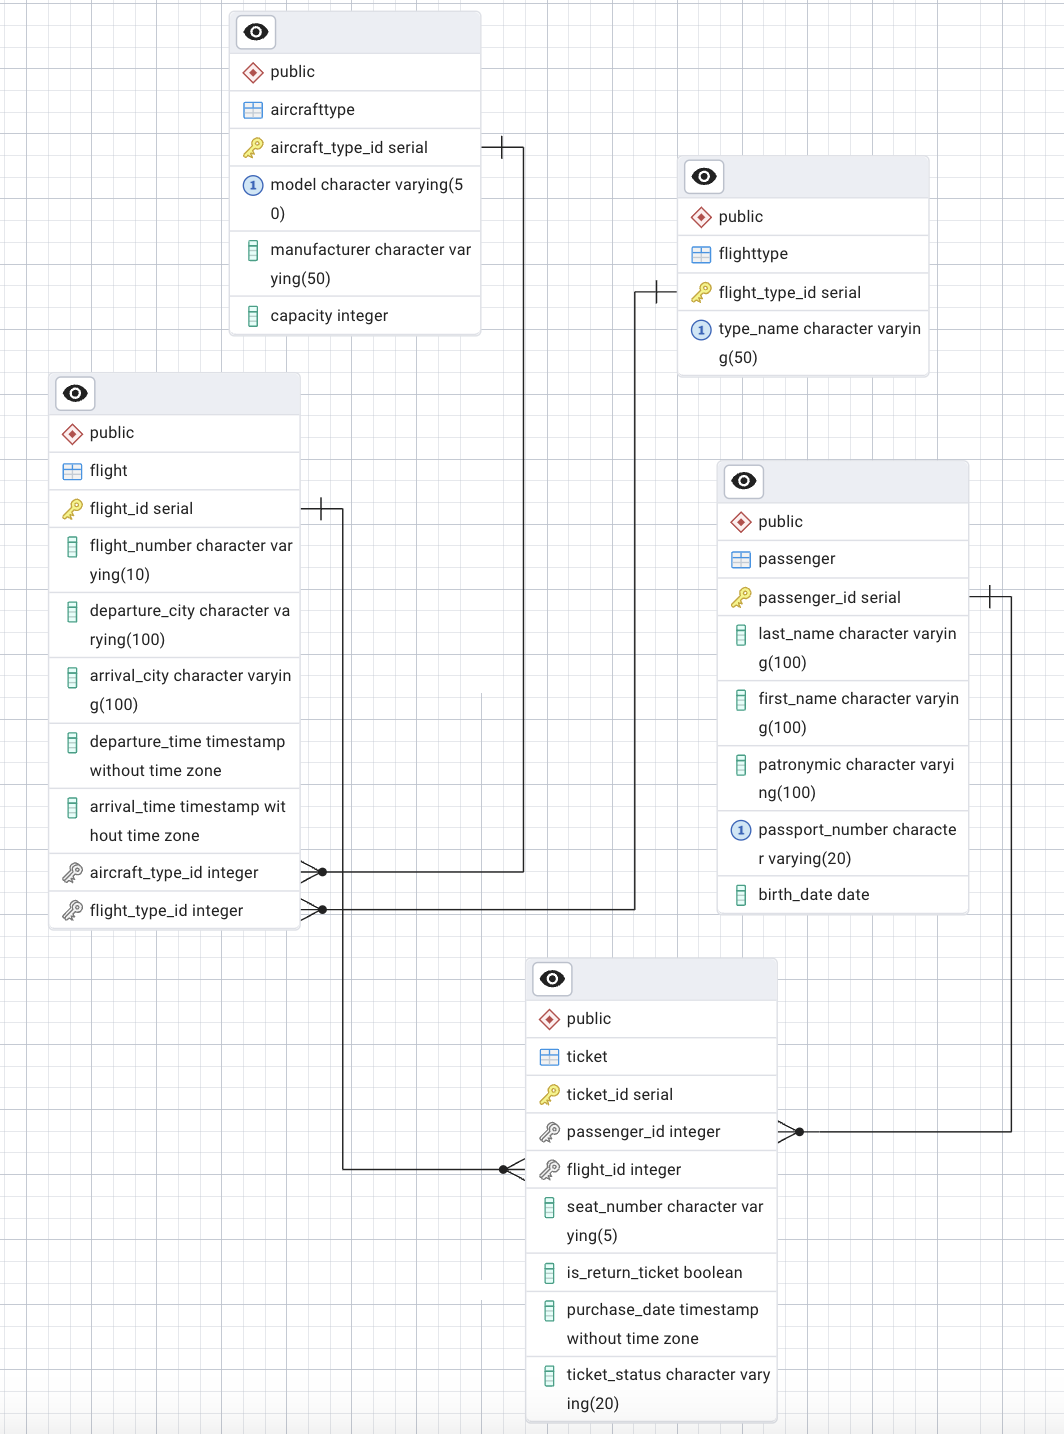
\includegraphics[width=0.8\textwidth]{DB_HW1.png}
\end{figure}

\section{Запросы на языке реляционной алгебры}

Обозначим отношения:
\begin{itemize}
    \item $Passenger$ — пассажиры
    \item $Flight$ — рейсы
    \item $Ticket$ — билеты
    \item $AircraftType$ — типы самолетов
    \item $FlightType$ — типы рейсов
\end{itemize}

\subsection*{Запрос 1: Список пассажиров заданного рейса}
Пусть задан рейс с номером '$SU100$':

\[
R_1 = Flight \bowtie Ticket \bowtie Passenger
\]
\[
Result = \pi_{LastName, FirstName, Patronymic, PassportNumber}(\sigma_{FlightNumber='SU100'}(R_1))
\]

\subsection*{Запрос 2: Пассажиры с обратным билетом до заданного города}
Пусть заданный город — 'Москва':

\[
R_1 = Flight \bowtie Ticket \bowtie Passenger
\]
\[
Result = \pi_{LastName, FirstName, Patronymic}(\sigma_{ArrivalCity='Moscow' \land IsReturnTicket=TRUE}(R_1))
\]

\subsection*{Запрос 3: Рейсы пассажира по фамилии и дате}
Пусть фамилия — 'Иванов', дата — '$2024-03-15$':

\[
R_1 = Passenger \bowtie Ticket \bowtie Flight
\]
\[
Result = \pi_{FlightNumber, DepartureCity, ArrivalCity, DepartureTime}
\]
\[
(\sigma_{LastName='Ivanov' \land DATE(DepartureTime)='2024-03-15'}(R_1))
\]

\subsection*{Запрос 4: Однофамильцы на одном рейсе}

\[
R_1 = Passenger \bowtie Ticket
\]
\[
R_2 = R_1 \times R_1
\]
\[
R_3 = \sigma_{R_1.LastName=R_2.LastName \land R_1.FlightID=R_2.FlightID \land R_1.PassengerID < R_2.PassengerID}(R_2)
\]
\[
Result = \pi_{R_1.LastName, R_1.FirstName, R_2.FirstName, R_1.FlightNumber, R_1.DepartureTime}(R_3)
\]

\subsection*{Запрос 5: Список свободных мест}

Для этого запроса необходимо ввести вспомогательное отношение $Seats$, содержащее все возможные номера мест:

\[
Seats = \pi_{SeatNumber}(\sigma_{SeatNumber\ IS\ NOT\ NULL}(Ticket))
\]

Тогда все возможные комбинации рейсов и мест:

\[
AllFlightSeats = Flight \times Seats
\]

Занятые места (билеты с указанными местами):

\[
OccupiedSeats = \pi_{FlightID, SeatNumber}(Ticket)
\]

Свободные места получаются вычитанием занятых из всех возможных:

\[
FreeSeats = AllFlightSeats \setminus OccupiedSeats
\]

Итоговый результат с проекцией на нужные атрибуты:

\[
Result = \pi_{DepartureDate, FlightNumber, Seat, DepartureCity, ArrivalCity}(FreeSeats \bowtie Flight)
\]

где $DepartureDate = DATE(DepartureTime)$.

\subsection*{Запрос 6: Пассажиры до заданного города в интервале дат}
Пусть заданный город — 'Сочи', интервал — с '$2024-03-01$' по '$2024-03-31$':

\[
R_1 = Flight \bowtie Ticket \bowtie Passenger
\]
\[
Result = \pi_{LastName, FirstName, Patronymic, FlightNumber, DepartureTime}
\]
\[
( \sigma_{ArrivalCity='Sochi' \land DepartureTime \ge '2024-03-01' \land DepartureTime \le '2024-03-31'}(R_1))
\]

\subsection*{Запрос 7: Типы самолетов по маршруту пассажира}
Пусть задан номер билета $ticket\_id = 1$:

Сначала найдем рейс, на который куплен данный билет:

\[
R_1 = \sigma_{TicketID=1}(Ticket) \bowtie Flight
\]

Из этого рейса получим маршрут (город отправления и прибытия):

\[
Route = \pi_{DepartureCity, ArrivalCity}(R_1)
\]

Теперь найдем все рейсы, выполняющиеся по этому маршруту:

\[
R_2 = Flight \bowtie Route
\]

И для этих рейсов получим типы самолетов:

\[
R_3 = R_2 \bowtie AircraftType
\]

\[
Result = \pi_{Model, Manufacturer}(R_3)
\]

\subsection*{Запрос 8: Три самых востребованных направления за месяц}
Пусть задан месяц — март 2024 года (год = 2024, месяц = 3):

Сначала отфильтруем рейсы за указанный месяц:

\[
MonthlyFlights = \sigma_{EXTRACT(YEAR FROM DepartureTime)=2024 \land EXTRACT(MONTH FROM DepartureTime)=3}
\]
\[
(Flight)
\]

Подсчитаем количество проданных билетов по каждому направлению:

\[
R_1 = MonthlyFlights \bowtie Ticket
\]

\[
DirectionCounts = \mathcal{G}_{DepartureCity, ArrivalCity; COUNT(DISTINCT TicketID) \rightarrow TicketCount}(R_1)
\]

Сортируем по убыванию количества и берем первые 3:

\[
SortedDirections = \tau_{TicketCount DESC}(DirectionCounts)
\]

\[
Result = \delta_{3}(SortedDirections)
\]

где $\mathcal{G}$ — оператор группировки с агрегатными функциями, $\tau$ — оператор сортировки, $\delta_{3}$ — оператор ограничения количества записей (TOP 3).

\section{Группы пользователей и ожидаемые запросы}

\subsection{Менеджер по продажам}
\begin{itemize}
    \item Сколько билетов продано на рейс SU100 за последнюю неделю?
    \item Какие пассажиры сегодня вылетают в Париж?
\end{itemize}

\subsection{Сотрудник службы безопасности}
\begin{itemize}
    \item Есть ли в списке пассажиров на рейс SU200 однофамильцы с подозреваемыми (заданный список фамилий)?
    \item Кто из пассажиров с фамилией Иванов летал за последний месяц?
\end{itemize}

\subsection{Аналитик}
\begin{itemize}
    \item Какие 3 направления были самыми популярными в прошлом месяце?
    \item Какой тип самолета чаще всего используется на рейсах в Новосибирск?
\end{itemize}

\subsection{Пассажир}
\begin{itemize}
    \item Есть ли свободные места на рейс SU300 завтра?
    \item Какие рейсы летят из Москвы в Сочи в ближайшую пятницу?
\end{itemize}

\section{Нормализация базы данных}

Спроектированная база данных соответствует \textbf{Третьей нормальной форме (3НФ)}.

\textbf{Обоснование:}
\begin{enumerate}
    \item \textbf{1НФ:} Все атрибуты атомарны. В таблице Passenger ФИО разбито на три отдельных поля. Даты и времена хранятся в стандартных типах данных SQL, что обеспечивает их неделимость в контексте данного отношения.
    
    \item \textbf{2НФ:} Таблицы находятся в 1НФ, и каждый неключевой атрибут функционально полно зависит от первичного ключа. В таблице Ticket неключевые поля (seat\_number, purchase\_date) зависят от всей связки (рейс + пассажир), а не от части ключа.
    
    \item \textbf{3НФ:} Таблицы находятся в 2НФ и не содержат транзитивных зависимостей. Например, в таблице Flight информация о модели самолета вынесена в отдельную таблицу AircraftType и связана через внешний ключ. Таким образом, departure\_city зависит только от flight\_id и не зависит от других неключевых атрибутов.
\end{enumerate}

\section{Скрипт создания таблиц на SQL}

\begin{verbatim}
-- Создаем таблицу типов самолетов
CREATE TABLE AircraftType (
    aircraft_type_id SERIAL PRIMARY KEY,
    model VARCHAR(50) UNIQUE NOT NULL,
    manufacturer VARCHAR(50) NOT NULL,
    capacity INTEGER NOT NULL CHECK (capacity > 0)
);

-- Создаем таблицу типов рейсов (справочник)
CREATE TABLE FlightType (
    flight_type_id SERIAL PRIMARY KEY,
    type_name VARCHAR(50) UNIQUE NOT NULL
);

-- Создаем таблицу пассажиров
CREATE TABLE Passenger (
    passenger_id SERIAL PRIMARY KEY,
    last_name VARCHAR(100) NOT NULL,
    first_name VARCHAR(100) NOT NULL,
    patronymic VARCHAR(100),
    passport_number VARCHAR(20) UNIQUE NOT NULL,
    birth_date DATE NOT NULL
);

-- Создаем таблицу рейсов
CREATE TABLE Flight (
    flight_id SERIAL PRIMARY KEY,
    flight_number VARCHAR(10) NOT NULL,
    departure_city VARCHAR(100) NOT NULL,
    arrival_city VARCHAR(100) NOT NULL,
    departure_time TIMESTAMP NOT NULL,
    arrival_time TIMESTAMP NOT NULL,
    aircraft_type_id INTEGER REFERENCES AircraftType(aircraft_type_id),
    flight_type_id INTEGER REFERENCES FlightType(flight_type_id)
);

-- Создаем таблицу билетов (связь пассажиров и рейсов)
CREATE TABLE Ticket (
    ticket_id SERIAL PRIMARY KEY,
    passenger_id INTEGER NOT NULL REFERENCES Passenger(passenger_id) ON DELETE CASCADE,
    flight_id INTEGER NOT NULL REFERENCES Flight(flight_id) ON DELETE CASCADE,
    seat_number VARCHAR(5),
    is_return_ticket BOOLEAN DEFAULT FALSE,
    purchase_date TIMESTAMP DEFAULT CURRENT_TIMESTAMP,
    ticket_status VARCHAR(20) DEFAULT 'Куплен',
    CONSTRAINT unique_flight_passenger UNIQUE (flight_id, passenger_id)
);

-- Индексы для ускорения поиска
CREATE INDEX idx_ticket_passenger ON Ticket(passenger_id);
CREATE INDEX idx_ticket_flight ON Ticket(flight_id);
CREATE INDEX idx_flight_datetime ON Flight(departure_time);
CREATE INDEX idx_passenger_name ON Passenger(last_name, first_name);

-- Инигиляция всех таблиц
-- DROP TABLE AircraftType, FlightType, Passenger, Flight, Ticket;
-- DROP TABLE IF EXISTS AircraftType, FlightType, Passenger, Flight, Ticket CASCADE;
\end{verbatim}

\section{Заполнение базы данных}

\begin{verbatim}
-- Заполняем справочники
INSERT INTO FlightType (type_name) VALUES 
    ('Регулярный'),
    ('Чартер'),
    ('Специальный');

INSERT INTO AircraftType (model, manufacturer, capacity) VALUES 
    ('Boeing 737-800', 'Boeing', 189),
    ('Airbus A320', 'Airbus', 180),
    ('Sukhoi Superjet 100', 'Sukhoi', 98);

-- Добавляем пассажиров
INSERT INTO Passenger (last_name, first_name, patronymic, passport_number, birth_date) VALUES
	('Иванов', 'Александр', 'Сергеевич', '1234 567898', '1990-05-15'),
    ('Иванов', 'Иван', 'Иванович', '1234 567890', '1990-05-15'),
    ('Петров', 'Петр', 'Петрович', '2345 678901', '1985-10-20'),
    ('Сидоров', 'Сидр', 'Сидорович', '3456 789012', '1978-03-10'),
    ('Иванова', 'Мария', 'Ивановна', '4567 890123', '1995-07-25'),
    ('Петров', 'Алексей', 'Иванович', '5678 901234', '1988-12-05'),
	('Иванов', 'Александр', 'Сергеевич', '1234 567899', '1990-05-15');

-- Добавляем рейсы
INSERT INTO Flight (flight_number, departure_city, arrival_city, departure_time, arrival_time, aircraft_type_id, flight_type_id) VALUES
    ('SU100', 'Москва', 'Санкт-Петербург', '2024-03-15 10:00:00', '2024-03-15 11:30:00', 1, 1),
    ('SU101', 'Санкт-Петербург', 'Москва', '2024-03-18 18:00:00', '2024-03-18 19:30:00', 1, 1),
    ('SU200', 'Москва', 'Сочи', '2024-03-16 14:00:00', '2024-03-16 16:30:00', 2, 1),
    ('SU201', 'Сочи', 'Москва', '2024-03-20 09:00:00', '2024-03-20 11:30:00', 2, 1),
    ('CH750', 'Москва', 'Анталья', '2024-03-17 23:00:00', '2024-03-18 04:00:00', 3, 2);

-- Продаем билеты
INSERT INTO Ticket (passenger_id, flight_id, seat_number, is_return_ticket, purchase_date) VALUES
    (6, 1, '1A', FALSE, '2024-02-02 11:20:00'),
    (1, 1, '12A', FALSE, '2024-02-01 10:00:00'),
    (2, 1, '12B', FALSE, '2024-02-01 10:05:00'),
    (1, 2, '10A', TRUE, '2024-02-01 10:00:00'), -- Обратный билет для Иванова
    (3, 3, '5F', FALSE, '2024-02-15 14:30:00'),
    (4, 3, '5E', FALSE, '2024-02-15 14:35:00'),
    (5, 3, '6A', FALSE, '2024-02-16 09:00:00'),
    (2, 5, '1A', FALSE, '2024-03-01 11:20:00');
\end{verbatim}

\section{Реализация отчетов}

\begin{verbatim}
-- 1. Получить список всех пассажиров заданного рейса (SU100)
SELECT p.last_name, p.first_name, p.patronymic, p.passport_number
FROM Passenger p
JOIN Ticket t ON p.passenger_id = t.passenger_id
JOIN Flight f ON t.flight_id = f.flight_id
WHERE f.flight_number = 'SU100';

-- 2. Пассажиры, вылетающие до заданного города и имеющие 
-- обратный билет (город = 'Москва')
SELECT DISTINCT p.last_name, p.first_name, p.patronymic
FROM Passenger p
JOIN Ticket t ON p.passenger_id = t.passenger_id
JOIN Flight f ON t.flight_id = f.flight_id
WHERE f.arrival_city = 'Москва' AND t.is_return_ticket = TRUE;

-- 3. Рейсы пассажира с заданной фамилией и датой вылета ('Иванов', '2024-03-15')
SELECT f.flight_number, f.departure_city, f.arrival_city, f.departure_time
FROM Flight f
JOIN Ticket t ON f.flight_id = t.flight_id
JOIN Passenger p ON t.passenger_id = p.passenger_id
WHERE p.last_name = 'Иванов' AND DATE(f.departure_time) = '2024-03-15';

-- 4. Однофамильцы на одном рейсе
SELECT p1.last_name, p1.first_name, p2.first_name AS namesake_firstname, 
       f.flight_number, f.departure_time
FROM Passenger p1
JOIN Ticket t1 ON p1.passenger_id = t1.passenger_id
JOIN Passenger p2 ON p1.last_name = p2.last_name 
AND p1.passenger_id < p2.passenger_id
JOIN Ticket t2 ON p2.passenger_id = t2.passenger_id AND t1.flight_id = t2.flight_id
JOIN Flight f ON t1.flight_id = f.flight_id;

-- 5. Список свободных мест (Дата, № рейса, № места, Город отправления, Город прибытия)
-- Генерируем все возможные места для рейса и вычитаем занятые
WITH seat_numbers AS (
    SELECT DISTINCT seat_number AS seat
    FROM Ticket
    WHERE seat_number IS NOT NULL
),
flight_seats AS (
    SELECT f.flight_id, f.flight_number, f.departure_city, f.arrival_city, 
           f.departure_time::DATE AS flight_date, s.seat
    FROM Flight f
    CROSS JOIN seat_numbers s
)
SELECT fs.flight_date AS "Дата", fs.flight_number AS "№ рейса", 
       fs.seat AS "№ места", fs.departure_city AS "Город отправления", 
       fs.arrival_city AS "Город прибытия"
FROM flight_seats fs
LEFT JOIN Ticket t ON fs.flight_id = t.flight_id AND fs.seat = t.seat_number
WHERE t.ticket_id IS NULL;

-- 6. Пассажиры, вылетавшие до заданного города в заданном интервале дат
-- (город = 'Сочи', интервал '2024-03-01' - '2024-03-31')
SELECT p.last_name, p.first_name, p.patronymic, f.flight_number, f.departure_time
FROM Passenger p
JOIN Ticket t ON p.passenger_id = t.passenger_id
JOIN Flight f ON t.flight_id = f.flight_id
WHERE f.arrival_city = 'Сочи' 
  AND f.departure_time BETWEEN '2024-03-01' AND '2024-03-31';

-- 7. Типы самолетов, летающих по тому же маршруту, 
-- что и самолет пассажира с заданным номером билета (ticket_id = 1)
SELECT DISTINCT at2.model, at2.manufacturer
FROM Ticket t1
JOIN Flight f1 ON t1.flight_id = f1.flight_id
JOIN AircraftType at1 ON f1.aircraft_type_id = at1.aircraft_type_id
JOIN Flight f2 ON f1.departure_city = f2.departure_city 
AND f1.arrival_city = f2.arrival_city
JOIN AircraftType at2 ON f2.aircraft_type_id = at2.aircraft_type_id
WHERE t1.ticket_id = 1;

-- 8. Три самых востребованных направления за указанный месяц
-- (март 2024)
SELECT f.departure_city AS "Город отправления", 
       f.arrival_city AS "Город прибытия", 
       COUNT(DISTINCT t.ticket_id) AS "Количество проданных билетов"
FROM Flight f
JOIN Ticket t ON f.flight_id = t.flight_id
WHERE EXTRACT(YEAR FROM f.departure_time) = 2024 
  AND EXTRACT(MONTH FROM f.departure_time) = 3
GROUP BY f.departure_city, f.arrival_city
ORDER BY COUNT(DISTINCT t.ticket_id) DESC
LIMIT 3;
\end{verbatim}

\end{document}